\documentclass[../../ClassicThesis.tex]{subfiles}
\begin{document}

\section{Computer Graphics in Web Environments}
\label{sec:cg-web}
% ************************************************

In this section we give a brief overview of graphics programming
fundamentals in general and in web environments. These fundamentals
are the concepts of {\threedmodel} data representation in
Section~\sectionref{sub:model-representation} and render loops and scene
graphs in Section~\sectionref{sub:render-and-graph}.

\subsection{3d~Model Representation}
\label{sub:model-representation}

This section explains the mesh data structure and the {\stlfile}
format that is used to represent {\threedmodel}s on disk.

The model geometry is represented by a set of connected
polygons, approximating the model surface. These connected
polygons form a mesh. Figure~\ref{fig:term-mesh:mesh} shows
a mesh. We use triangles as polygons, because they
benefit from hardware acceleration. A triangle in the mesh
is called face. Figure~\ref{fig:term-mesh:face} illustrates
the terminology. Each face is described by a list of three
points in 3D~space. Such a point is called vertex. A single
vertex is described by three floating point numbers for the
x-, y- and z-coordinates. An edge is the line between two
connected vertices \cite[p.~3]{intro-cg}.

\begin{figure}[h]
  \centering
  \begin{subfigure}[b]{0.49\textwidth}
    \centering
    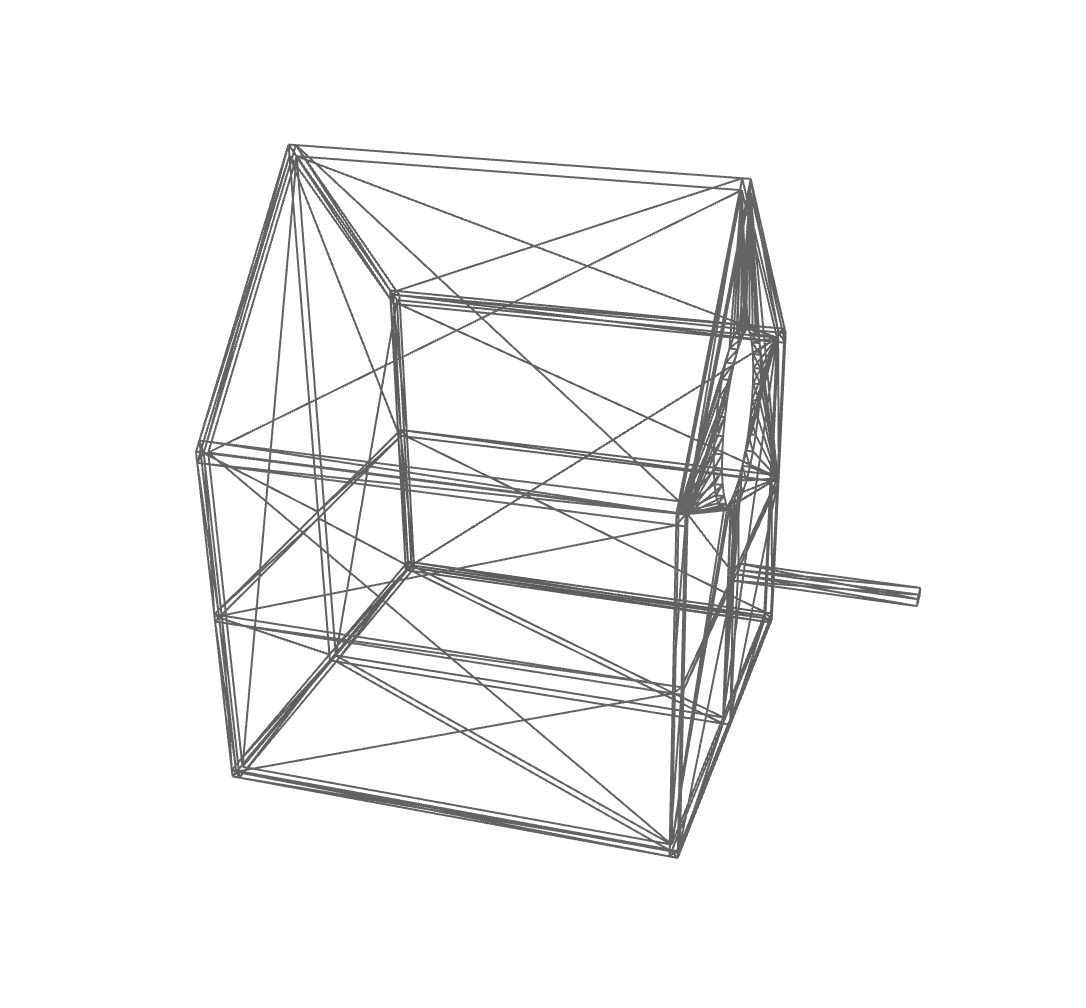
\includegraphics[width=\textwidth]{03-architecture-birdhouse}
    \caption{A triangle mesh of a bird house.}
    \label{fig:term-mesh:mesh}
  \end{subfigure}
  \begin{subfigure}[b]{0.49\textwidth}
    \centering
    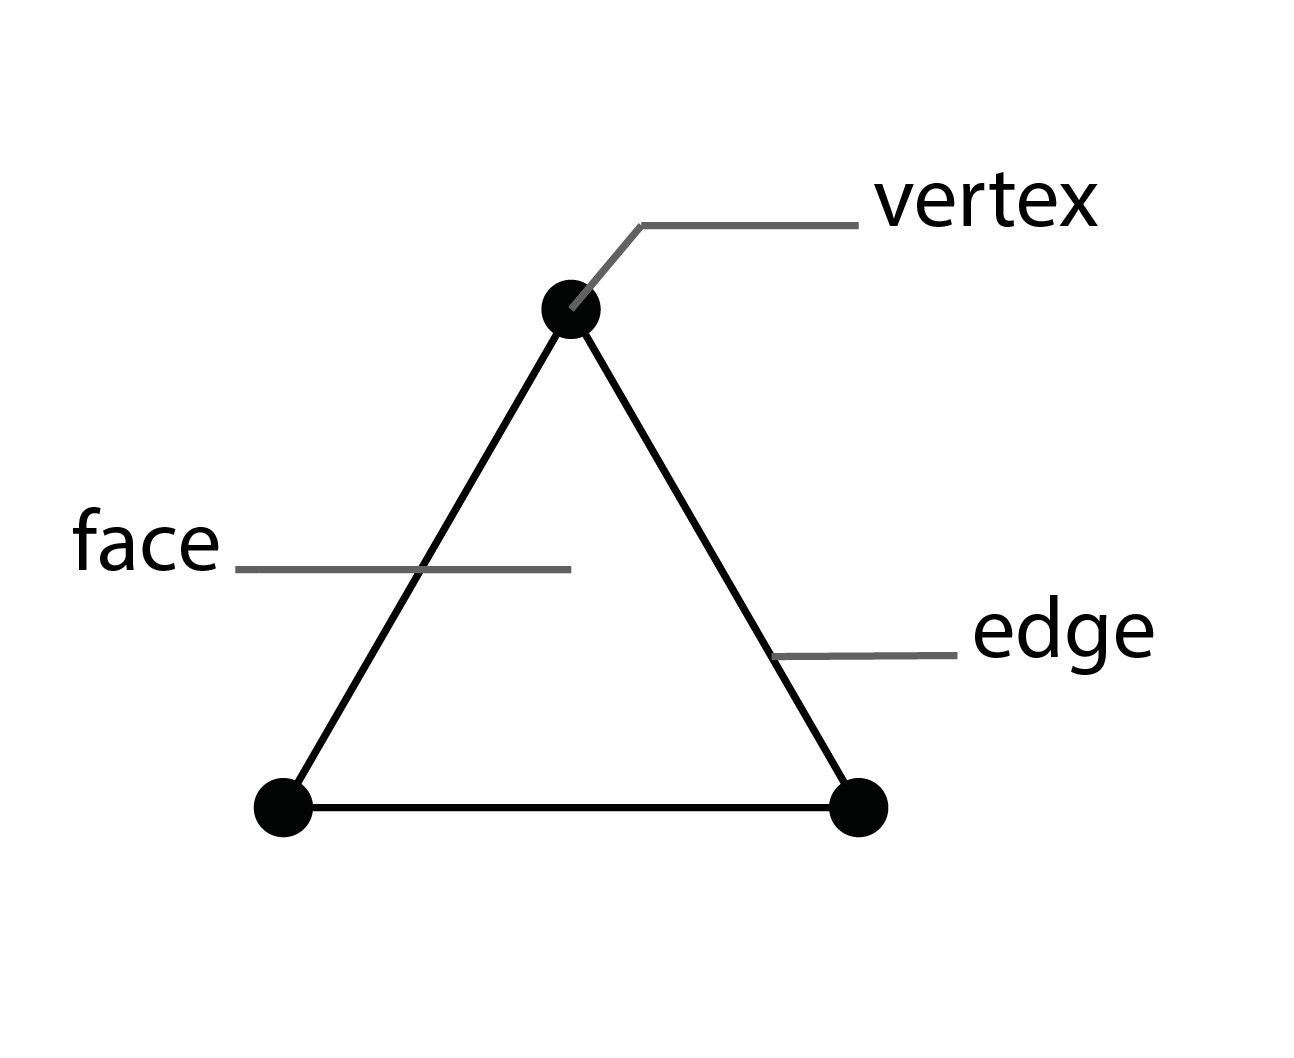
\includegraphics[width=\textwidth]{03-architecture-mesh-terminology}
    \caption{A single face with vertices and edges.}
    \label{fig:term-mesh:face}
  \end{subfigure}
  \caption{Terminology of a Mesh}
  \label{fig:term-mesh}
\end{figure}

{\platener} supports all geometry which is arranged in two-manifold
meshes. Two-manifoldness is a constraint on the mesh, which requires
each egde to exactly touch two neighboring faces.
Figure~\ref{fig:non-manifold} shows a non-manifold part of a mesh.
Each triangular face of a two-manifold mesh has to have three adjacent
faces. This constraint enforces the mesh to be a fully connected graph
without holes \cite[p.~28]{master-thesis}. In order to make
sophisticated assumptions when designing the conversion algorithms,
the software requires two-manifold meshes.

\begin{figure}[h]
  \centering
  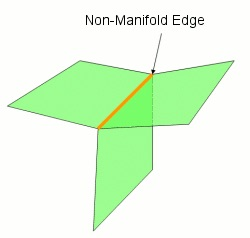
\includegraphics[width=0.6\textwidth]{03-architecture-non-manifold}
  \caption{A non-manifold cut-out of a mesh.}
  \label{fig:non-manifold}
\end{figure}

We load {\threedmodel}s in the Standard Tessellation
Language (STL) format. STL is a common file format for
{\threedmodel} representation in the context of
{\threedprinting}. The reason we focus on the STL format is
the possibility to make 3D printer formats available for the
laser cutter. An {\stlfile} consists of a list of faces
associated with their face normal. Each face is given as a
list of vertices. We cannot say in which direction the face
points judging only from the vertices. The face normal
determines the orientation of the face.
Listing~\ref{alg:stl-file} shows an {\stlfile} in ASCII
encoding. An {\stlfile} can also be stored in a binary
format. The binary format is commonly used because it
requires less disk-space than the ASCII encoding
\cite[p.~8]{stl-file}.

\begin{listing}
\begin{verbatim}
solid name
 facet normal n1 n2 n3
  outer loop
  vertex p1x p1y p1z
  vertex p2x p2y p2z
  vertex p3x p3y p3z
  endloop
 endfacet
endsolid name
\end{verbatim}
\caption{General format of a STL-file in ASCII encoding.}
\label{alg:stl-file}
\end{listing}

% Reconstructing the original {\threedmodel} from an
% {\stlfile} does not always result in an one-to-one solution.
The vertices are stored as floating point numbers. Two faces
that share the same vertex refer to that vertex by
floating point numbers as well. Due to rounding errors the
same vertex can be represented by slightly different
floating point numbers. Without a look-up table, in which
vertices are referred to by a unique index, vertices cannot
be distinguished fail-safe. We have to assume that two
overlapping points represent an identical vertex. We use the
library
{\meshlib}\footnote{\url{https://github.com/brickify/meshlib}}
to create an indexed face-vertex mesh from the possibly
ambiguous {\stlfile}. The face-vertex mesh is converted to a
{\threejs} geometry by {\meshlib}. With a {\threejs}
geometry we can render a {\threedmodel} in {\convertify}.

To support a variety of {\threedprinter} optimized models,
we use the {\stlfile} format. We import the files with the
{\meshlib} library. The imported face-vertex mesh structure
is then converted for usage with {\threejs}. The section
below explains how the {\threejs} representation is
displayed on the screen.

\subsection{Render Loop and Scene Graphs}
\label{sub:render-and-graph}

To understand how {\convertify} and {\platener} work, we
have to familiarize ourselves with the concepts of rendering
and scene graphs first.

A typical pattern in graphics software is the render loop.
Rendering is the process of turning the {\threedmodel}
representation into an array of pixels which can be
displayed on the screen~\cite[p.~2]{intro-cg}. A
{\threedmodel} is rendered in a continuous loop to produce
an interactive experience rather than a single static image.
The render loop pattern consists of three steps: processing
input, updating the {\threedmodel} representation and
rendering~\cite{gamedev-gameloop}.
Figure~\ref{fig:render-loop} shows an exemplary flow.

\begin{figure}[h]
  \centering
  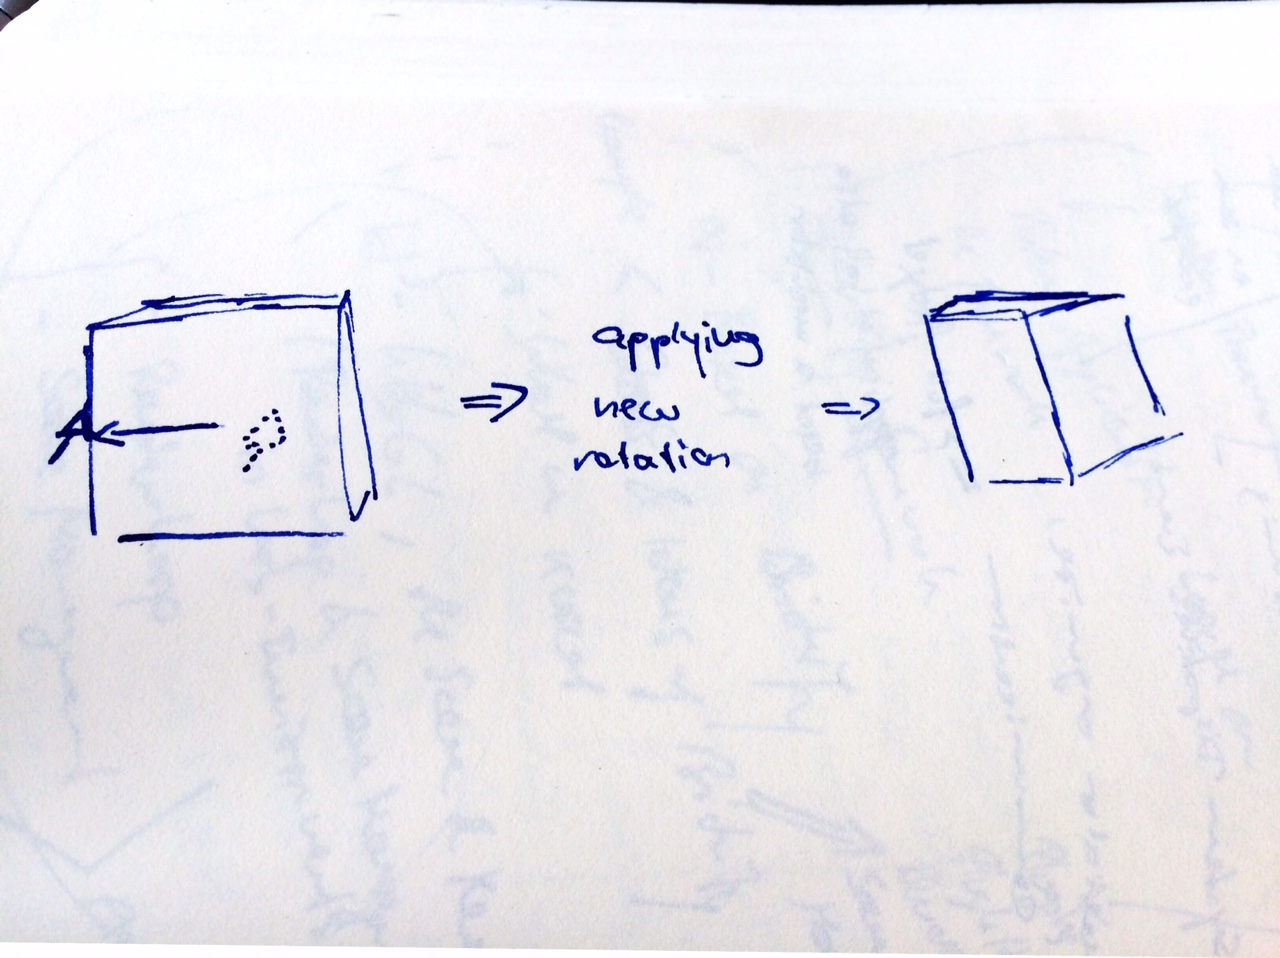
\includegraphics[width=1\columnwidth]{03-architecture-render-loop}
  \caption{Pointer input is processed by the render loop.}
  \label{fig:render-loop}
\end{figure}

Each object is part of a scene. A scene is the visual space,
in which the rendered objects can be seen. We use
representations of objects which are organized in a
hierarchical tree data structure. We refer to this
hierarchical structure as scene graph~\cite{scene-graph}. A
simple scene graph is depicted in
Figure~\ref{fig:scene-graph}. The graph contains a box as
single root node. The sides of the box are children of the
root node. With this abstraction transformations are applied
to parts of the model only, without necessarily touching
each face or vertex. Every object that is recognized by
{\convertify} is part of a scene graph. Finally, the
vertices of an object in the scene graph are rendered to the
screen.

\begin{figure}[H]
  \centering
  \begin{subfigure}[b]{0.49\textwidth}
    \centering
    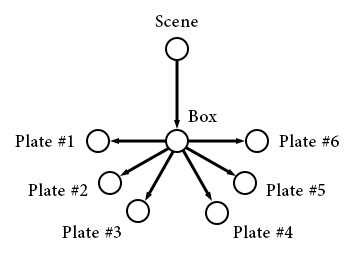
\includegraphics[width=\textwidth]{03-architecture-scene-graph-abstract}
    \caption{Graph notation of the composed box.}
    \label{fig:scene-graph:abstract}
  \end{subfigure}
  \begin{subfigure}[b]{0.49\textwidth}
    \centering
    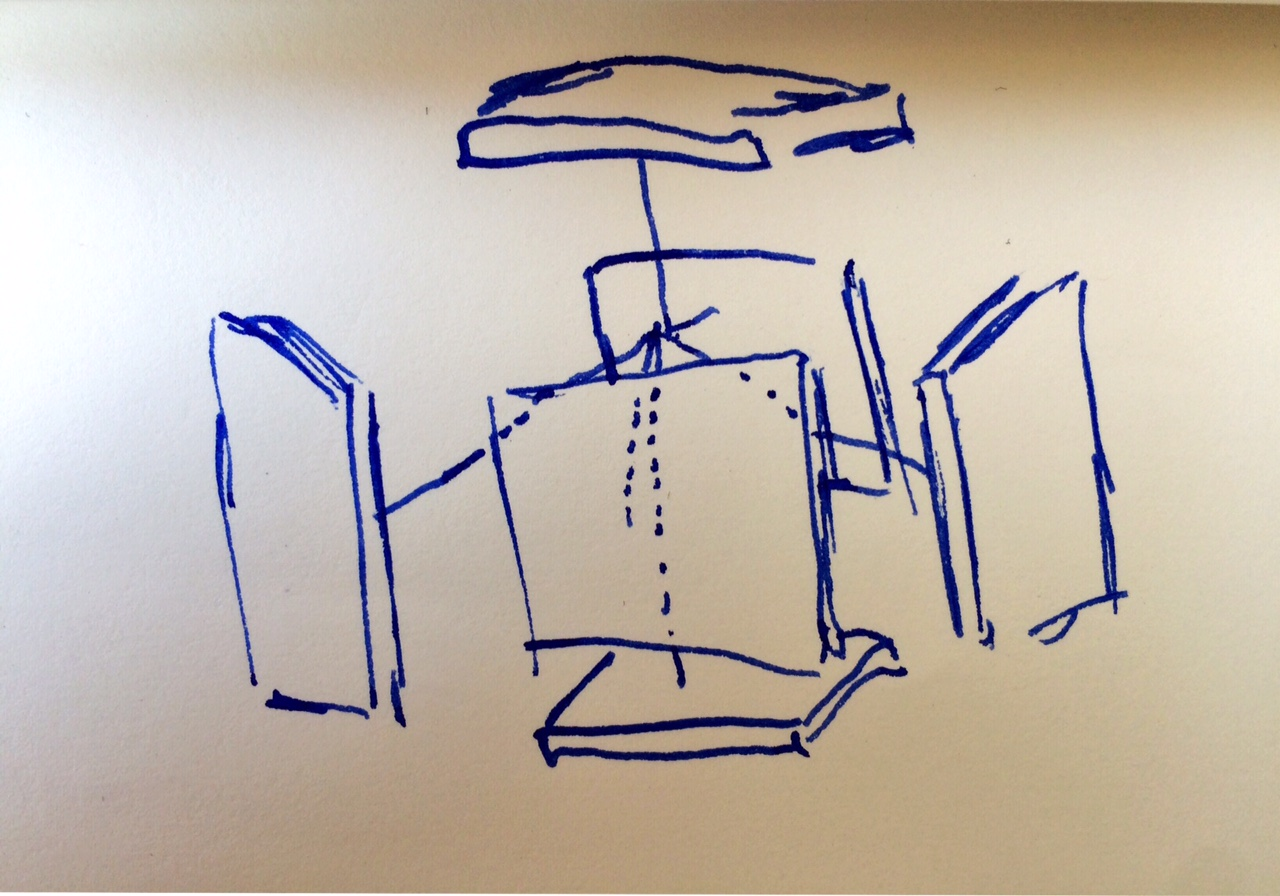
\includegraphics[width=1\textwidth]{03-architecture-scene-graph-visual}
    \caption{Rendered box in an explosion view, showing decomposition into plates.}
    \label{fig:scene-graph:visual}
  \end{subfigure}
  \caption{A scene graph showing a box, composed of plates.}
  \label{fig:scene-graph}
\end{figure}


The framework {\convertify} uses common computer graphics
patterns like render loops and scene graphs. With the help
of WebGL and {\threejs} we are able to bring these concepts
into a web environment.

\end{document}

%%% Local Variables:
%%% mode: latex
%%% TeX-master: "../../ClassicThesis"
%%% TeX-command-extra-options: "-shell-escape"
%%% End:
